% !TEX root = ../thesis-example.tex
%
\chapter{Metodologia}
\label{Metodologia}

Descripcion de metodo aplicado para entropia  ver diagrama \ref{diagramaentropia1}.

Para comenzar, los datos se han obtenido a través del portal Yahoo Finance, por lo que son registros del precio de cierre de cada dia, además dichos datos fueron depurados y ordenados ya que había algunos espacios en blanco en el archivo original, entonces el software con que se trabaja interpreta los datos sin errores. 

Luego que se han cargado los datos, y se han ordenado es necesario calcular los retornos de los precios. La razón por la que se trabajan los retornos de los precios y no se trabaja directamente con los precios ya que no poseen estacionaridad en el tiempo y ello conlleva a que no va a haber una media central en los datos. Los retornos permiten que los datos se encuentren entorno a una media.

Aunque los retornos son una mejor representación de los precios, aún presentan picos que sobresalen de la media, por lo que se estandarizan los retornos, la estandarización permitirá destacar aquellos retornos que realmente poseen picos en su valor de retorno. 

Ya que cada retorno ha sido estandarizado con su respectiva fecha,  se procede a discretizar los retornos mediante un proceso que divide en cuatro intervalos a los retornos. Determinar los cuartiles de los retornos y discretizarlos con base en la etiqueta que se pone a cada intervalo, en otras palabras, los intervalos van a permitir etiquetar del 1 al 4 a cada retorno. 

La ecuación de la entropía requiere conocer la probabilidad de los elementos del sistema, con los intervalos dados por los cuartiles y la discretización de los retornos se obtiene todo lo necesario para calcular la entropía, sin embargo, no se calcula la entropía de todo el conjunto de datos, se hace por subconjuntos de datos agrupados en listas de 50 elementos, o cualquier número dado por el usuario.

El resultado de la entropia es dado en valores y fechas para cada subconjunto de días.

\begin{figure}
	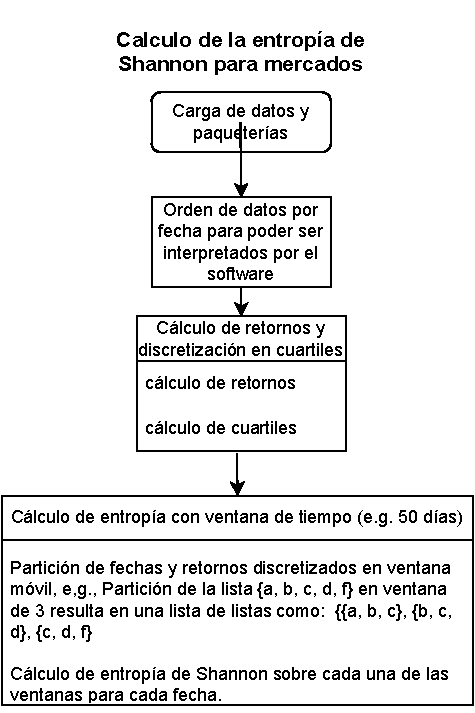
\includegraphics[width=0.7\linewidth]{figures/diagrama_entropia1}
	\caption{Diagrama del algoritmo utilizado para el c\'alculo de entrop\'ia de Shanon en mercados financieros.}
	\label{diagramaentropia1}
\end{figure}


Descripcion de metodo aplicado para entropia utlizando medias moviles ver Figura \ref{entropiamav} . 
Se aplica el mismo metodo mencionado arriba, adicionalmente en la etapa en que se estandarizan los retornos de los precios con su respectiva fecha. La ventana puede ser elegida por el usuario. Se aplica una entrada de por lo menos 50 días ya que un número menor no suavizaría la curva de manera que no se podría apreciar tendencias en el comportamiento de la curva.





\begin{figure}
	\centering
	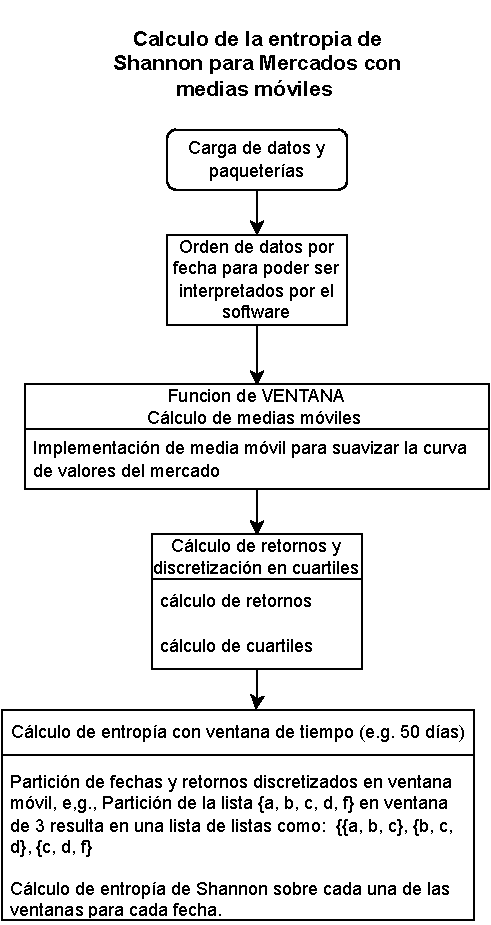
\includegraphics[width=0.7\linewidth]{figures/entropiaMAV}
	\caption{Diagrama del algoritmo utilizado para el c\'alculo de entrop\'ia de Shanon en mercados financieros con medias m\'oviles.}
	\label{entropiamav}
\end{figure}

La simulación de un mercado eficiente requiere cargar datos debido a que se simula un caminante aleatorio a partir de una distribución gaussiana con una media y desviación estándar obtenidas del análisis de los retornos (no estandarizados) de los precios reales. 

Del paso anterior se obtienen retornos simulados, mismos que deben estandarizarse y asignarles su fecha.

A partir de este punto hay dos situaciones que se pueden apreciar en el diagrama \ref{simulacion}, la primera es que a dichos retornos simulados se les aplica el proceso para el cálculo de entropía de la figura \ref{diagramaentropia1}, y la segunda es que se aplica el proceso de medias móviles como se presenta en \ref{entropiamav}.


Se destacan valores mínimos de entropía gracias a la manera en que se presentan los resultados, con ello comparar el comportamiento de la entropía del mercado eficiente y del mercado real con fechas, con o sin media móvil requiere únicamente del cálculo de un umbral que diferencie los valores de entropía que se comportan de manera gaussiana  de los que no.

Mediante la definición de un umbral que permite seleccionar con un intervalo de confianza de 95 porciento los valores de entropía mínima en los mercados. 

\begin{figure}
	\centering
	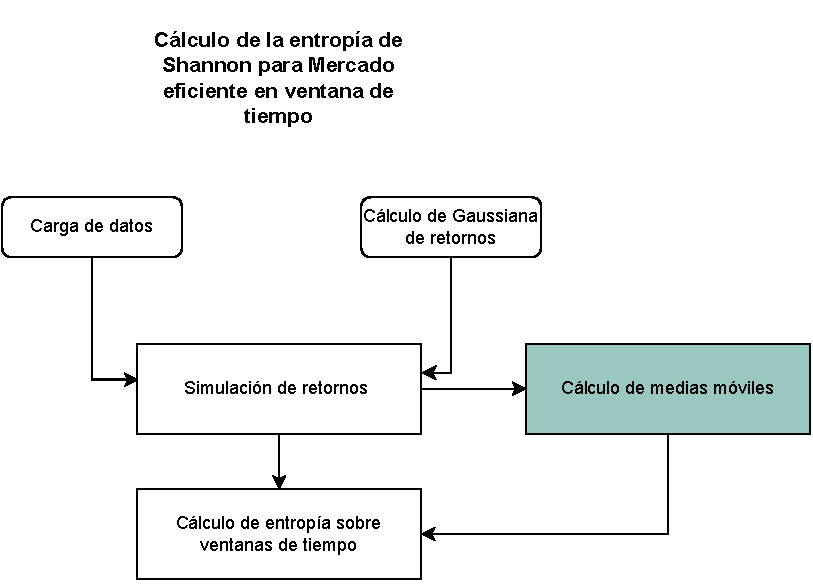
\includegraphics[width=0.9\linewidth]{figures/simulacion}
	\caption{Diagrama del algoritmo de calculo de entropia para la simulacion de mercado eficiente. }
	\label{simulacion}
\end{figure}

Reglas de cuartiles
\begin{center}
	\begin{tabular}{ |r | l | c| }
		 \hline
		Cuartil & Regla & etiqueta \\
		primer cuartil & $\inf > 0$ & 1 \\
		2 &   & Calculo de madia moviles utilizando N dias\\ 
		3 &     &Estimacion gaussiana con sigma igual 3 \\
		 \hline
	\end{tabular}
\end{center}



Finalmente, se aplica una prueba estadística de distribuciones a los valores con mínima entropía, tanto de aquellos que fueron tratados con un filtro de media movil como aquellos que no. 